\documentclass[times, utf8, zavrsni,numeric,pstricks]{fer}
\graphicspath{{lib/pics/}} %Setting the graphicspath

\definecolor{codegreen}{rgb}{0,0.6,0}
\definecolor{codegray}{rgb}{0.5,0.5,0.5}
\definecolor{codepurple}{rgb}{0.58,0,0.82}
\definecolor{backcolour}{rgb}{0.95,0.95,0.92}
\lstdefinestyle{mystyle}{
    backgroundcolor=\color{backcolour},   
    commentstyle=\color{codegreen},
    keywordstyle=\color{magenta},
    numberstyle=\tiny\color{codegray},
    stringstyle=\color{codepurple},
    basicstyle=\ttfamily\footnotesize,
    breakatwhitespace=false,         
    breaklines=true,                 
    captionpos=b,
    keepspaces=true,                 
    showspaces=false,                
    showstringspaces=false,
    showtabs=false,                  
    tabsize=4  
}

%command for vector boldness
\newcommand{\vect}[1]{\boldsymbol{#1}}
%\newcommand{\engl}[1]{\textit{#1}}
%
%\engl{treast}

\lstset{style=mystyle}

\begin{document}

% TODO: Navedite broj rada.
\thesisnumber{000}

% TODO: Navedite naslov rada.
\title{Prepoznavanje emocija iz izraza lica pomoću strojnog učenja}

% TODO: Navedite vaše ime i prezime.
\author{Matej Ciglenečki}

\maketitle

% Ispis stranice s napomenom o umetanju izvornika rada. Uklonite naredbu \izvornik ako želite izbaciti tu stranicu.
\izvornik

% Dodavanje zahvale ili prazne stranice. Ako ne želite dodati zahvalu, naredbu ostavite radi prazne stranice.
\zahvala{}

\tableofcontents

\chapter{Uvod}

Većina komunikacije među ljudima je neverbalna. Ton glasa, geste, govor tijela i izrazi lica često vjernije prenose informacije od riječi. Običaji, način govora i kontekst trenutačne situacije govor čine podložnim mnoštvu različitih interpretacija dok je neverbalna komunikacija intuitivnija i univerzalnija. Ljudski dojmovi o drugim ljudima stvoreni su iz naoko suptilnih ali itekako važnih oblika neverbalne komunikacije. Saznanja i objašnjenja kognitivnih procesa iza ovih krajnje uobičajenih pojava još uvijek se aktivno istražuju. 

Strojno učenje se zadnjih godina počelo primjenjivati na probleme poput razumijevanje govora, raspoznavanje objekata na slikama i ostalim područjima koje su za čovjeka intuitivne i lake. Računalni vid kao novija grana znanosti u nekoliko godina naišla je na mnoštvo otkrića i inovacija. Susret sa računalnim vidom događa se gotovo svakodnevno, od kamera i sustava sposobnih za prepoznavanje lica koji su se počeli implementirati od strane mnogih država do personaliziranih filtara za lice popularne na društvenim mrežama. Jedan od takvih izazova računalnog vida je raspoznavanje ljudskih emocija na temelju izraza lica. Iako uporaba ove tehnologije još nije izašla u širu primjenu trenutno već postoje slučajevi gdje se ova tehnologija pokazala korisnom. Automobil s mogućnošću prepoznavanjem emocija može upozoriti vozača kad je umoran ili pod većim nesvjesnim stresom kako ne bi dovodio sebe i druge sudionike u prometu u opasnost. Raspoznavanje emocija nalazi primjeni i u razgovorima za posao. Kvalitetno treniran model objektivniji je od ljudskog ispitivača koji može imati subjektivne predrasude zbog čega u nekim slučajevima model može točnije procijeniti emocije osobe koju se ispituje, rezultirajući u bolji uvid u ponašanje i karakteristike osobe. Nadalje, ovakva se tehnologija može koristiti i u istraživanju tržišta. Mišljenjem korisnika o proizvodima dobivena putem razgovora i anketa često su netočna ili iskrivljena zbog nedostatka spomenute neverbalne komunikacije. Analiza emocija korisnika za vrijeme interakcije s proizvodom puno je reprezentativniji pokazatelj korisnikovog mišljenja. 

**Poreba za prepoznavanjem emocija**
**što emocije govore**
**gdje se koristi prepozavanje emocija**
**korištena metoda za klasifikaciju emcoija**



%Prijenosnim učenjem moguće je istrenirani model koji može klasificirati ljudske emocije uz određenu točnost, ovisno o pristupu kojeg koristimo prilikom odabira skupa podataka pomoću kojeg treniramo model.
%
%Odabrani skup podataka Cohn-Kanade koji sadrži sekvence slika ljudskih emocija i njihove označene emocije. Prije samog treniranja potrebno je procesirati i urediti podatke te stvoriti jedinku svake slike koja u sebi ima sve potrebne labele nužne za što bolje stvoren model. To je uređen par (sadržaj slike, emocija, FACS podatak). Pošto za pojedinu sekvencu znamo samo o kojoj se emociji radi potrebno je linearno sklairati neutralnu emociju i emociju o kojoj se radi tako da svaka slika uistinu reprezentira o kojoj se kombinacija emocija radi.



\chapter{Podatkovni skup}
\section{Uvod}
Podatkovni skup sastavni je dio u izvedbi treniranja modela. Treniranje se svodi na ulazne i izlazne podatke gdje su ulazni podaci podskup podatkovnog skupa. Korišteni podatkovni skupovi su Cohn-Kanade (CK) i skup slika preuzetih sa Google-a na temelju ključne riječi. Podatkovni skup dijelimo na dva djela. Skup za treniranje i skup za testiranje. Svi podaci koji su u skupu za treniranje iskorištavaju se za treniranje i optimiziranje odabranog modela dok se skup za testiranje koristi samo za evaluaciju točnosti treniranog modela. 80\% nasumičnih slika odabrane su za treniranje a ostalih 20\% koristi se za evaluaciju.

\section{Extended Cohn-Kanade podatkovni skup}

Cohn-Kanade podatkovni skup sastoji se od 593 sekvenci slika od 123 subjekta (osoba). Pojedina sekvenca sastoji se od 10 do 60 slika. Početna slika u sekvenci je neutralna emocija dok je zadnja slika vrhunac izraza emocije. Subjekti na slikama imaju od 18 do 50 godina, 69\% su žene, 81\% euro-Amerikanci i 6\% su subjekti ostalih rase. Rezolucija pojedine slike iznosi 640x480 ili 640x490 piksela u 8-bitnom crno-bijelom ili 24 bitnom puno-bojnom formatu\cite{ck}.

\begin{figure}[H]
	\includegraphics[width=\linewidth]{ck_example.png}
	\caption{Primjer slike iz CK+ podatkovnog skupa}
	\label{Podatkovni skup}
\end{figure}

\section{Ručno generirani podatkovni skup}
Slike CK+ podatkovnog skupa slikane su u istom okruženju (ista prostorija u kojoj se slikaju subjekti, ista kamera, slična svjetlina slike...). Nedostatak raznolikosti među slikama stvara potrebu za uvođenjem apstraktnijih slika ljudskih lica ne bi li model klasificirao emocije ljudskih lica koja nisu slična samo CK+ podatkovnom skupu. Zbog toga se uvodi podatkovni skup Google slika. Google omogućuje pretraživanje slika po zadanom upitu te dodatnim parametrima koji olakšavaju pronalaženje ljudskog lica koji predstavlja određenu emociju. Npr. pronalazak ljudskih lica koji iskazuju tužnu emociju mogao bi biti "sad human face" sa tipom Google slike "lice". Rezultati tog upita prikazani su na slici \ref{pic:google_search_sad}.

\begin{figure}[H]
	\includegraphics[width=\linewidth]{2020-06-08-22-16-22.jpeg}
	\caption{Rezultati Google upita "sad human face"}
	\label{pic:google_search_sad}
\end{figure}

Rezultati ovog upita su slike veće raznolikosti (različit scenarij i drugačiji kut gledanja) što pridonosi apstrakciji emocije u ukupnom podatkovnom skupu. Dobivene slike ne odgovaraju uvijek nužno zadanom upitu zbog čega je potrebno dodatno provjeriti valjanost pojedine slike. Proces filtriranja objašnjen je u poglavlju \ref{google_npy_filter}


\section{Priprema podatkovnih skupova}\label{priprema_ck}
\subsection{Priprema Cohn-Kanade podatkovnog skupa}
\subsubsection{Struktura podataka}

Dijelovi podatkovnog skupa značajni za treniranje dijele se na direktorij sekvence i emocije. Svaki subjekt (npr. S005) ima svoj direktoriji u kojem se nalaze pod direktoriji za emociju koju je subjekt odglumio (npr. 001, 002...) a u njemu se nalaze sekvence. Za 327 sekvenca postoji odgovarajuća emocija koja je definirana samo za krajnju sliku sekvence i njezina putanja je definirana jednako kao i za sekvencu.

\pagebreak

\begin{figure}[H]
\centering
\begin{Verbatim}[fontsize=\small]
├── emotions
│   ├── S005
│   │   └── 001
│   │       └── S005_001_00000011_emotion.txt
│   │       	└── "3.0000000e+00"
│   ├── S010
│   │   ├── 001
│   │   ├── 002
│   │   │   └── S010_002_00000014_emotion.txt
│   │   │   	└── "4.0000000e+00"
│   │   └── ...
│   └── ...
└── images
    ├── S005
    │   └── 001
    │       ├── S005_001_00000001.png
    │       ├── ...
    │       └── S005_001_00000011.png
    ├── S010
    │   ├── 001
    │   │   ├── S010_001_00000001.png
    │   │   ├── ...
    │   │   └── S010_001_00000013.png
    │   ├── 002
    │   │   ├── S010_002_00000001.png
    │   │   ├── ...
    │   │   └── S010_002_00000014.png
    │   └── ...
    └── ...

\end{Verbatim}
\caption{Struktura podataka CK+ podatkovnog skupa}
\label{cb:npy_tree}
\end{figure}

\subsubsection{Obrada podataka}
Jedina slika u sekvenci za koju je definirana emocija je zadnja slika, što znači da je potrebno je potrebno odrediti vektor emocije ostalih slika u sekvenci na temelju krajnje vrijednosti emocije. Emocija za pojedinu sliku definirana je kao red emocija. Svaki indeks reda predstavlja emociju kojih ima kojih ima 8. Indeks pojedine emocije definiran je na slici \ref{cb:emo_declare} a vrijednost na indeksu predstavlja intenzitet emocije

\begin{figure}[H]
\centering
\begin{Verbatim}[fontsize=\small]
emocije = {
    1: "neutral",
    2: "anger",
    3: "contempt",
    4: "disgust",
    5: "fear",
    6: "happy",
    7: "sadness",
    8: "surprise",
}
\end{Verbatim}
\caption{Deklaracija emocija}
\label{cb:emo_declare}
\end{figure}

\noindent
Znajući da je emocija za početnu sliku neutralna a za krajnju maksimalna sekvencijska emocija, emocije za ostale slike dodijeljene su linearno na način da se odredi intenzitet neutralne emocije \ref{eq:intensity_neutral} i sekvencijske emocije \ref{eq:intensity_seq} gdje je $n$ ukupan broj slika u sekvenci a $i$ slika kojoj se određuje vektor emocije.

\begin{equation}\label{eq:intensity_neutral}
	p_{n} = \dfrac{i-1}{n-1}	
\end{equation}
\begin{equation}\label{eq:intensity_seq}
\begin{split}
	p_{s} = 1 - p_{n}\\
	p_{s} + p_{n} = 1	
\end{split}
\end{equation}

\subsubsection{Primjer vektora emocije za sekvencu "disgust" koja sadrži 10 slika:}

\begin{figure}[H]
\centering
\begin{tabular}{|c|c|} 
\hline
broj slike & vektor emocije \\
\hline
$i = 1$ & [1.0, 0.0, 0.0, 0.0, 0.0, 0.0, 0.0, 0.0] \\
... & ... \\
$i = 6$ & [0.4, 0.0, 0.0, 0.6, 0.0, 0.0, 0.0, 0.0] \\
... & ... \\
$i = n = 10$ & [0.0, 0.0, 0.0, 1.0, 0.0, 0.0, 0.0, 0.0] \\
$i$ & [$p_n$, 0.0, 0.0, $p_s$, 0.0, 0.0, 0.0, 0.0]  \\
\hline
\end{tabular}
\caption{Vektor emocije za pojedinu pojedinu sliku u sekvneci u CK podatkovnom skupu}
\label{pic:ck_emotion_rise}
\end{figure}



\subsubsection{Spremanje slike i vektora emocije u .npy podatak}\label{self:npy_save}
Za daljnje korištenje svaka slika i njezin vektor emocije će pretvorena u numpy red \cite{numpy_array} i spremljen kao .npy podatak. Prvi element numpy reda je slika a drugi je odgovarajući vektor emocije. Ovime je osigurano da izračun emocija za pojedinu sliku je izračunat samo jedanput što će smanjiti vrijeme potrebno za treniranje. Nakon provođenja transformacije podataka u .npy podatak ukupan broj slika i pripadajućih vektora emocija iznosi 5703. 



\begin{figure}[H]\label{fig:npy_array}
	\begin{subfigure}[b]{0.5\linewidth}
	  	\centering
		\includegraphics[width=\linewidth]{numpy_slika_emocija.png}
		\caption{Struktura .npy podatka}		
	\end{subfigure}
	\begin{subfigure}[b]{0.5\linewidth}
	  	\centering
		\includegraphics[width=\linewidth]{numpy_imgdata_emo.png}
		\caption{Sadržaj .npy podatka}
	\end{subfigure}	
	\caption{.npy podatak}	
\end{figure}


\subsection{Priprema Google podatkovnog skupa}\label{priprema_google}
\subsubsection{Prikupljeni podaci}
Umjesto preuzimanja jedne po jedne slike korištena je google-images-download skripta \cite{google-images-download} koja preuzima sve moguće slike na temelju zadanog upita. Upiti korišteni za pronalaženje odgovarajućih emocija nalaze se na slici \ref{cb:google_queries} a svi su popraćeni dodatnim "Google search" parametrom koji pretražuje slike samo ljudskih lica. Svaka slika spremljena je u direktoriji čije je ime upit koji je bio korišten prilikom preuzimanje te slike. 

\begin{figure}[H]
	\centering
		\begin{Verbatim}[fontsize=\small]
		"sad human face"
		"neutral human face"
		"neutral expression"
		"angry human face"
		"angry expression"
		"contempt"
		"fear human face"
		"fear expression"
		"surprise human face"
		"surprise expression"
		"disgusted human face"
		"disgust expression"
		\end{Verbatim}
	\caption{Upiti za preuzimanje ljudskih lica sa Google-a}
	\label{cb:google_queries}
\end{figure}

\noindent
Nakon preuzimanja svih mogućih slika potrebno je ručno proći kroz svaki direktorij svakog upita i izbaciti slike koje ne zadovoljavaju sljedeće uvjete \label{google_npy_filter}

\begin{itemize}
	\item Na slici se nalazi samo jedno ljudsko lice
	\item Na slici se nalazi ljudsko lice čija emocija odgovara upitu pomoću kojeg je slika preuzeta
	\item Veličina slike je manja od 20MB
	\item Rezolucija slike je veća od 20px po duljini i visini
	\item Slika nije duplikat prethodno viđene slike
	\item Slika nije dio CK+ podatkovnog skupa
\end{itemize}
Uklanjanjem slika koje ne zadovoljavaju bilo koje od navedenih uvjeta dobiven ukupan broj slika povoljnih za treniranje iznosi 3160 a njihova ukupna veličina je 2,3GB.

\subsubsection{Struktura podataka}
Nakon filtriranja slika nepogodnih za treniranje potrebno je objediniti upite čiji su rezultati ljudska lica efektivno istih emocija. Primjer takva dva upita su "neutral human face" i "neutral expression". Nakon objedinjavanja rezultata upita i preimenovanja direktorija stvorena je struktura podataka dana na slici \ref{cb:google_file_structure}


\begin{figure}[H]
\centering
\begin{Verbatim}[fontsize=\small]
├── neutral
│   ├── 1.57053528-man-head-shot.png
│   ├── 2.Face_of_SpooSpa.png
│   ├── 3.main-1-low-res-4a61d.png
│   └── ...
├── anger
│   ├── 1.57053528-man-head-shot.png
│   └── ...
├── contempt
│   └── ...
├── disgust
│   └── ...
├── fear
│   └── ...
├── happy
│   └── ...
├── sadness
│   └── ...
└── surprise
    └── ...
\end{Verbatim}
\caption{Struktura podataka Google podatkovnog skupa}
\label{cb:google_file_structure}
\end{figure}

\subsubsection{Obrada podataka}
Obrada Google podatkovnog skupa bit će manje zahtjevna od CK+ podatkovnog skupa zbog toga što će se vektor emocije za pojedinu sliku odrediti samo na temelju upita korištenog za preuzimanje slike. Rezultat svakog vektora emocije bit će vektor dobiven metodom "One hot encoding". "One hot encoding" je metoda dodjele binarne vrijednosti za kategoriju u koju neki uzorak pripada ili ne pripada\cite{one_hot_encoding}. Ovom metodom uzorak (slika) može pripadati samo jednoj kategoriji (emocija). Slika koja pripada određenoj emociji za tu će emociju imati vrijednost 1 a za sve ostale 0. Na slici \ref{pic:google_emotion_emo_vector} prva kolumna označava ime direktorija u kojem se slike nalaze, druga kolumna predstavlja vektor emocije koje će slike u direktoriju poprimiti.

\begin{figure}[H]
\centering
\begin{tabular}{|c|c|} 
\hline
emocija (ime direktorija) & vektor emocije \\
\hline
neutral & [1,0,0,0,0,0,0,0] \\
anger	& [0,1,0,0,0,0,0,0] \\
contempt & [0,0,1,0,0,0,0,0] \\
disgust & [0,0,0,1,0,0,0,0]\\
fear  & [0,0,0,0,1,0,0,0]\\
happy & [0,0,0,0,0,1,0,0]\\
sadness & [0,0,0,0,0,0,1,0]\\
surprise & [0,0,0,0,0,0,0,1]\\
\hline
\end{tabular}
\caption{Vektor emocije za pojedinu emociju u Google podatkovnom skupu}
\label{pic:google_emotion_emo_vector}
\end{figure}

\subsubsection{Spremanje slike i vektora emocije u .npy podatak}
Nakon dodjele vektora emocije za pojedinu sliku potrebno je pretvoriti sliku i vektor emocije u .npy podatak. Kako se radi o slici i vektoru emocije, postupak pretvorbe slike i vektora emocije u pojedinačni .npy podatak jednak je kao i kod CK+ podatkovnog skupa definiranom u poglavlju \ref{self:npy_save}.


\subsection{Objedinjavanje podatkovnih skupova}
Nakon obrade CK+ i Google podatkovnog skupa svi .npy podaci bit će spremljeni u direktoriji "ck" ili "Google" ovisno o tome iz kojeg je podatkovnog skupa slika dobivena. Struktura svih .npy podataka prikazana je na slici \ref{pic:npy_structure}. Ovom strukturom moguće je definirati udio svakog podatkovnog skupa koji će biti korišten za treniranje modela. Poslije podjele u zasebne direktorije potrebno je odvojiti dio .npy podataka u test pod-direktoriji. U njemu će se nalaziti 10\% svih .npy podataka koji će modelu biti neviđeni prilikom treniranja. Tih 10\% .npy podataka koristit će se pri evaluaciji točnosti modela.


\begin{figure}[H]
\centering
\begin{Verbatim}[fontsize=\small]
numpy
├── ck
│   ├── test
│   │	├── test_slika_i_emocija_0001.npy
│   │	├── ...
│   │	└── test_slika_i_emocija_0570.npy
│   ├── slika_i_emocija_0001.npy
│   ├── ...
│   └── slika_i_emocija_5133.npy
└── google
    ├── test
    │	├── test_slika_i_emocija_0001.npy
	│	├── ...
	│	└── test_slika_i_emocija_0316.npy
    ├── slika_i_emocija_0001.npy
    ├── ...
    └── slika_i_emocija_2844.npy
    

\end{Verbatim}
\caption{Struktura .npy podataka}
\label{pic:npy_structure}
\end{figure}



\chapter{Treniranje}
Treniranje je proces u kojem model postupno mijenja svoje parametre ne bi li došao do idealnih parametara, čime bi model optimalno služio onome čemu je namijenjen. U slučaju klasifikacije za treniranje je potrebno imati skup podataka nad kojim će se provoditi treniranje i labele tih podataka koje govore klasu podataka. U slučaju klasifikacije emocija, skup podataka nad kojim se trenira su slike ljudskih lica dok je klasa emocija koja je prikazana na pojedinoj sliku. Kad treniranje započne, u model se pošalju podaci za koje model pokušava predvidjeti koje su klase ubačeni podaci. Nakon toga potrebno je usporediti predviđanja klasa koje je stvorio model sa pravim klasa. Pogrešku koju je model napravio prilikom predviđanja potrebno je javiti modelu ne bi li ispravio parametre. Mijenjanjem modela parametra model postaje sve bolji za predviđanje predviđanje rezultata na skupu za treniranje. Bitno je naglasiti da daljnjim treniranjem model ne postaje bolji za općeniti slučaj predviđanja. Treniranjem model se prilagođava podatkovnom skupu za treniranje. Podatkovni skup za treniranje je podskup svih podataka za koje je model namijenjen a to znači da skup za treniranje nije nužno najbolja mjera općenitog slučaja za podatke. 


Treniranje modela nakon određenog trenutka može pogoršati sposobnost modela da predviđa klase na općenitom slučaju. Uzrok toga je što treniranjem nakon točke TODO:NAME model ima veću točnost na skupu za treniranje ali točnost na općenitim, neviđenim slučajevima postaje sve manja. Zbog toga je potrebno pronaći optimalan trenutak u kojem treba prekinuti treniranje modela. Prekidanje treniranja modela nije moguće odrediti pomoću točnosti modela na skupu za treniranje jer ta točnost neprestano raste daljnjim treniranjem. Zbog toga je potrebno uvesti validacijski skup koji neće biti korišten prilikom treniranja. Validacijski skup o tom slučaju igra ulogu neviđenih podataka nad kojima se mjeri točnost. Prilikom treniranja točnost nad validacijskim skupom će rasti do točke TODO:ANME. U tom trenutku točnost nad validacijskim skupom će biti maksimalna a daljnjim treniranjem točnost će se smanjivati jer model postaje previše prilagođen skupu za treniranje \engl{overfitting}. 

TODO: slika - skup podataka  
**načini treniranja**

\section{Duboke neuronske mreže za analizu slika}
\subsection{Neuron}
Neuron je osnovni dio neuronske mreže. Svaki neuron na svoj ulaz prima vektor $x$ vrijednosti za koje neuron predviđa $\hat{y}$ izlaz. Skup $x$ vrijednosti je također pomnožen sa vektorom $w$ koji predstavlja težine \engl{weights} i zbrojen sa vrijednošću $b$ koja predstavlja sklonost \engl{bias}


\begin{equation}\label{eq:neuron_z}
	\vect{z}=w_1x_1+w_2x_2+...+w_nx_n=\vect{w^{T}} \cdot \vect{x}
\end{equation}

\begin{equation}\label{eq:neuron_func}
	\hat{y} = g(vect{z})
\end{equation}

\subsubsection{Aktivacijska funckija}

Nakon zbrajanja kroz neuron izlaz je potrebno provesti kroz aktivacijsku funkciju određuje koliko je signal tog neurona bio zastupljen u ukupnom izlazu, tj. koliko je "aktiviran". Cilj koji se postiže tom funkcijom je da ukupan izlaz neurona bude između vrijednosti 0 i 1. Dakle to su funkcije za koje vrijedi \ref{eq:activation_fun_general}. Primjer takvih funckija je sigmoid prikazan na slici \ref{fig:sigmoid} i rektifikacijska funckija \textit{(ReLU - engl. Rectifier)} prikazana na slici \ref{fig:relu}. Prilikom aktivacije neurona koristiti će se rektifikacijska funckija

\begin{equation}\label{eq:activation_fun_general}
	f:\mathbb{R} \rightarrow [0,1]
\end{equation}

\begin{figure}[H]
	\centering
		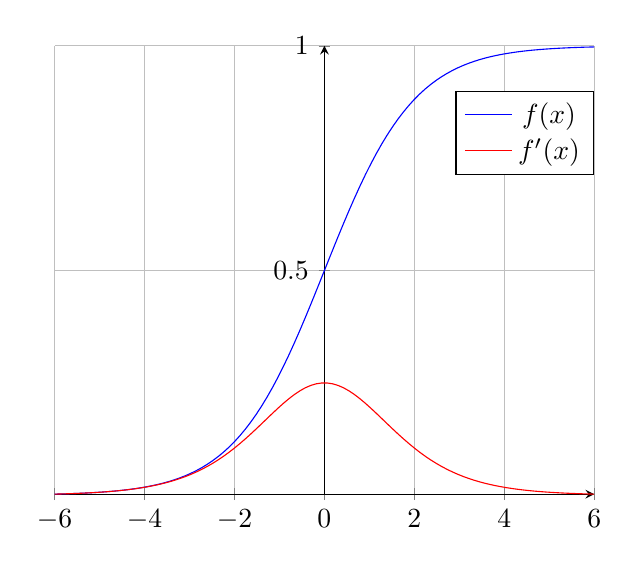
\begin{tikzpicture}[declare function={
			sigma(\x)=1/(1+exp(-\x));
			sigmader(\x)=sigma(\x)*(1-sigma(\x));
			},scale=1]
			
			\begin{axis}%
			[
			    grid=major,     
			    xmin=-6,
			    xmax=6,
			    axis x line=bottom,
			    ymax=1,
			    axis y line=middle,
			    ytick={0,.5,1},
			    samples=100,
			    domain=-6:6,
			    legend style={at={(1,0.9)}}     
			]
			    \addplot[blue,mark=none]   (x,{sigma(x)});
			    \addplot[red,mark=none]   (x,{sigmader(x)});
			    \legend{$f(x)$,$f'(x)$}
			\end{axis}
			\end{tikzpicture}
		\caption{Sigmoid}	
		\label{fig:sigmoid}	
\end{figure}		

\begin{figure}[H]
	\centering
		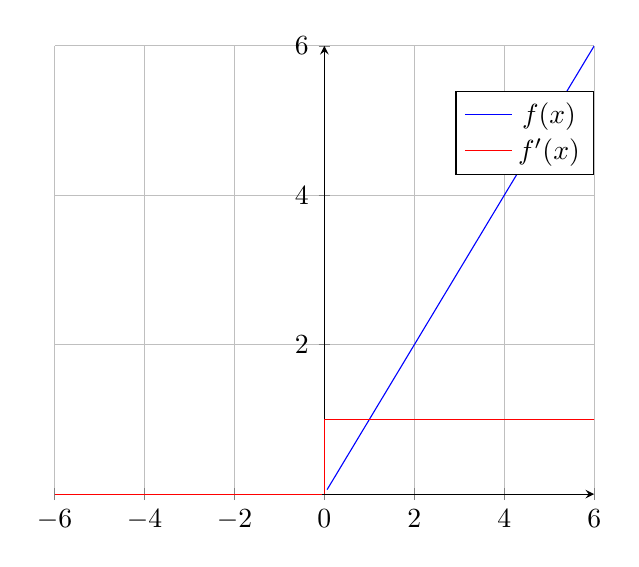
\begin{tikzpicture}[declare function={
			linear(\x)=\x;
			linearder(\x)=\x;
			},scale=1]
			
			\begin{axis}%
			[
			    grid=major,     
			    xmin=-6,
			    xmax=6,
			    axis x line=bottom,
			    ymax=6,
			    axis y line=middle,
			    samples=100,
			    domain=-6:6,
			    legend style={at={(1,0.9)}}     
			]	
			   \addplot[blue, restrict expr to domain={}{0:inf}]  (x,{linear(x)});
				\addplot[blue,  forget plot, restrict expr to domain={}{-inf:0}]  (x,0);
				\addplot[red, restrict expr to domain={}{-inf:0}]  (x,0);
				\addplot[red, const plot]  coordinates {(-inf,0) (0,0) (0,1) (100,1)};
			   \legend{$f(x)$,$f'(x)$}
			\end{axis}
			\end{tikzpicture}
		\caption{Linearna rektifikacijska funkcija}
		\label{fig:relu}
\end{figure}

\subsection{Sloj neurona}

Sloj neurona sastoji se od skupa neurona. Sloj neurona sastoji se od vektora $a$ koji označava aktivaciju sloja neurona. U slučaju prvog sloja vrijedi $a = x$. Račun izlaza sloja neurona računa se slično kao i kod pojedinog neurona. Za svaki sloj neurona $l$ izlaz $z$ jednak je umnošku prethodne aktivacije $a_{l-1}$ sa trenutnim težinama sloja neurona $w_l$ zbrojen sa sklonošću $b_l$


\begin{equation}\label{eq:neuron_layer}
	\boldsymbol{\vect{z_l}} = \vect{w_l} \cdot \vect{a_{l-1}} + \vect{b_l}
\end{equation}

\begin{equation}\label{eq:neuron_layer_func}
	\hat{y} = g(z)
\end{equation}

\subsection{Neuronska mreža}



Neuronska mreža sastoji se od više slojeva neurona koji su međusobno povezani. Slojevi su povezani tako da je svaki neuronski sloj razine $l$ povezan sa svakim neuronskim slojem razine $l+1$. Povezani su na način da se izlaz neuronskog sloja $l$ dovodi na ulaz neuronskog sloja $l+1$. Ovaj algoritam prijenosa podataka s jednog sloja na drugi zove se \textit{feedforward} algoritam. TODO: slika slojeva. Slojevi se dijele u tri različite grupe: ulazni, skriveni i izlazni sloj. Ulazni sloj je prvi sloj na koji se dovodi ulazni podataka, slika. Izlazni sloj je sloj koji na izlazu daje klasifikaciju ulazne slike, u ovom slučaju vektor predviđenih emocija. Skriveni slojevi su među-slojevi koji obrađuju podatke prethodnog izlaznog sloja neurona. Što je neuronski sloj dublje razine to je apstrakcija podataka koju on računa veća. Izlaz skrivenog sloja poslat će se na ulaz sljedećeg skrivenog sloja a tim prijelazom apstrakcija podataka će biti uvećana. Uloga svakog neuronskog sloja je da obrađuje podatke na razini apstrakcije definiranje njegovom dubinom. Većim brojem slojeva neurona stvara se dublja neuronska mreža koja može računati na većoj razini apstrakcije. Interpretacija razine apstrakcije u slučaju slika svodi se na promatranje različitih djelova slike različite veličine. Iako se promatraju različiti dijelovi slike, međuzavisnost neuronskih slojeva omogućava neuronskoj mreži da zna koje je svojstvo slike proizašlo iz prethodnog svojstva slike. Primjer bi bio pronalaženje ruba usnice i ruba oka na slici. Iako ta dva rubovi izgledom mogu biti slični bitna je spoznaja da jedan rub proizlazi iz slike usnice a drugi iz slike oka. TODO: slika usnica oko, sličan rub.


\subsection{Funkcija gubitka}
Funkcija gubitka \engl{Loss function} je funkcija koja govori koliko je neuronska mreža daleko ili blizu rezultata koji se želi postići. Rezultat funkcije gubitka bit će pogreška koju je mreža napravila prilikom predviđanja vektora emocije određene slike. Taj rezultat bit će korišten za ispravljanje parametara neuronske mreže. Funkcija gubitka treba ukazati na kojim je predviđanjima neuronska mreža pogriješila i za koliko. Križni entropijski gubitak \engl{Cross Entropy Loss} je funkcija gubitka dana sa \ref{eq:cross_entropy} koja će biti korištena prilikom određivanja gubitka. Funkcija prima dva parametra, ispravna vrijednost označenu kao vektor $x$ je i predviđenu vrijednost označenu kao vektor $y$. U slučaju predviđanja emocija $x$ je stvaran vektor emocije za pojedinu sliku dok je $y$ previđen vektor emocije stvoren kao izlaz neuronske mreže. Vektor $w$ predstavlja težišta za pojedini element vektora $x$ i $y$. Elementi vektora $w$ su $w_1, w_2, ..., w_n$ gdje svaki $w_i$ predstavlja koeficijent koji će biti pomnožen sa rezultatom gubitka. Razlog uvođenja težišta je neravnomjerna zastupljenost klasa u podatkovnom skupu za treniranje. Klase s manjim brojem uzoraka imat će veće težište prilikom računanja gubitka i samim time će biti "bitnije" prilikom treniranja. Kazna pogreške predviđanja za tu klasu tj. emociju bit će veća nego u slučaju ne korištenja težišta.

\begin{equation}\label{eq:cross_entropy}
	CrossEntropyWeighted\left(\vect{x}, \vect{y},\vect{w}\right) =
		-\sum_i w_i \left( x_i log\left(y_i \right)\right)
\end{equation}

\subsection{Treniranje neuronske mreže}

Neuronska mreža predstavlja nelinearnu funkciju koja se sastoji od mnogo parametara. To su spomenuti parametri pojedinog neurona spomenuti na formuli \ref{eq:neuron_z}, težišta neurona $\vect{w}$2 i sklonost neurona $b$. Mijenjanje tih parametra parametra na način da se rezultat funkcije gubitka smanjuje naziva se treniranje. Cilj treniranja je minimizirati gubitak na način da se pronađe lokalni minimum u $n$ dimenzionalnom prostoru, gdje je broj $n$ broj težina u neuronskoj mreži. Metoda pronalaska minimuma zove se spuštanje gradijentom \engl{gradient descent}. Računanje spusta svodi se na izračun derivacije parametra neuronske mreže prema \ref{eq:graident_der} gdje je greška neuronskog sloja $E$, $a$ aktivacijski izlaz  i $w$ težina sloja.

\begin{equation}\label{eq:graident_der}
	\frac{\partial E}{\partial w} = \frac{\partial E}{\partial a} \cdot \frac{\partial a}{\partial w}
\end{equation}

Ovom jednadžbom dobiven je smjer negativnog gradijenta koji vodi ka minimumu n dimenzionalne plohe. Brzina kojom neuronska mreža konvergira prema minimumu označena sa $lr$ zove se stopa učenja \engl{learning rate}. Gradijent se računa prilikom svake iteracije treniranja, tj. nakon svakog dovođenja slike na ulaz mreže. Izračunati gradijent na sloju $l_i$ pomnožen sa stopom učenja $lr$ povratnom vezom se šalje na prethodni sloj $l_{i-1}$. Sloj $l_{i-1}$ koristiti će dobivenu vrijednost da ažurira svoja težišta sljedećim izračunom:

\begin{equation}\label{eq:gradient_backprop_layer}
	 w_{l_{i-1}} - lr \frac{\partial E_{l_i}}{\partial w_{l_i}} \rightarrow w_{l_{i-1}}
\end{equation}

Ovaj postupak naziva se backpropagration i primjenjuje se na sve slojeve neurona u neuronskoj mreži.

..........
**stohasitcki ne ide uvijek prema minimumum**
**nakon svakog ulaza se racuna**
**lokalni minimum =/= pravi**

c

**općenito**2
**problem treniranja dubokih mreža**	
**gradient degradation problem**

4
\subsection{Rezidualna neuronska mreža}

Problem prilikom treniranja duboke neuronske mreže je mogućnost nestajućeg gradijenta \engl{vanishing gradient} pri ranim neuronskim slojevima mreže. Prilikom backprogragation algoritma sloj $l_i$ ažurirat će svoja težišta danom formulom \ref{eq:gradient_backprop_layer}. Bitno je naglasiti da vrijednost koja će ažurirati njegovo težište $lr \frac{\partial E_{l_n}}{\partial w_{l_n}}$ je gradijent izračunat od svih prethodnih slojeva $l_i+1, ..., l_n$


\subsection{Prijenosno učenje}

Prijenosno učenje je tehnika u području strojnog gdje je naučenost modela za predviđanje jednog cilja prenesena na predviđanje drugog cilja. Potreba za ovom tehnikom javlja se iz nedovoljno velikog skupa podataka korištenog za treniranje. Zbog toga što podatkovni skup nije dovoljno velik, neuronska mreža neće biti dovoljno trenirana da predviđa emocija za neviđene slike. Unaprijed trenirana neuronska mreža ResNet 50, koja je trenirana na ImageNet podatkovnom skupu \cite{imagenet_cvpr09}, omogućava mreži da od početka prepoznaje bitne značajke neviđene slike. Time je izbjegnuta potreba za treniranjem modela od početka jer su početni neuronski slojevi mreže već dobro naučeni za prepoznavanje bitnih značajki u slici, poput istaknutih objekta i uočljivijih oblika.

Zadnji slojevi unaprijed trenirane ResNet 50 mreže mogu predviđati 1000 različitih značajki. Broj mogućih klasifikacijskih emocija je 8 zbog čega će biti potrebno dodati zadnji neuronski sloj na postojeću neuronsku mrežu tako da izlaz mreže bude dimenzije 8, a ne 1000 što odgovara broju različitih klasa korištenih u ImageNet podatkovnom skupu. Korištenjem većeg i apstraktnijeg podatkovnog skupa ova se tehnika može izostaviti.

\section{Implementacija treniranja u PyTorch-u}
U poglavlju \ref{priprema_ck} i \ref{priprema_google} objašnjeno su iz oba podatkovna skupa dobiveni .npy podaci koji sadrže podatke slike i odgovarajućeg vektora emocije te slike. Sljedeći korak je iskoristiti te podatke za treniranje neuronske mreže koja će klasificirati emocije neviđenih slika ljudskih lica.

\subsection{Priprema podataka}
.npy podatke učitani su iz strukture definirane na \ref{pic:npy_structure}. Parametrima GOOGLE\_TRAIN\_SPLIT i CK\_TRAIN\_SPLIT moguće je kontrolirati koji će udio slika iz pojedinog podatkovnog skupa biti zastupljen u ukupnom skupu za treniranje.

\begin{figure}[H]
\centering
\begin{Verbatim}[fontsize=\small]
GOOGLE_TRAIN_SPLIT = 1
CK_TRAIN_SPLIT = 1
\end{Verbatim}
\caption{Udio .npy podataka pojedinog podatkovnog skupa}
\label{pic:split_dataset}
\end{figure}
\noindent
Sljedeći korak je implementacija klase Dataset iz PyTorch biblioteke. Stvaranjem klase FERDataset iz klase Dataset poslana su tri argumenta: lokacija .npy podataka i funkcija za transformaciju slika. FERDataset sad ima pristup lokaciji .npy podataka i preko te lokacije će dohvaćati .npy podatke prilikom treniranja.


\begin{figure}[H]
\centering

\begin{Verbatim}[fontsize=\small]
class FERDataset(Dataset):
    def __init__(self, filepaths_numpy, transform_image=None):
        self.filepaths_numpy = filepaths_numpy
        self.transform_image = transform_image
\end{Verbatim}
\caption{Definiranje FERDataset inicijalizacije}
\label{pic:init_dataset}

\end{figure}

\noindent
Nakon dohvata .npy podataka preko funkcije \_\_getitem\_\_ potrebno ga je raspakirati u sliku lica i vektor emocije te slike. Ukoliko je zadana transformacija slike ona će se primijeniti nakon raspakiravanja .npy podataka. Više o transformaciji slika bit će rečeno kasnije. 

\begin{figure}[H]
\centering

\begin{Verbatim}[fontsize=\small]
def __getitem__(self, idx):
        name_npy = filepaths_npy(idx)
        image, emotion = load_npy(name_npy)
        image = transform(image)
        return image, emotion
\end{Verbatim}
\caption{Pojednostavljeni dohvat i raspakiravanje .npy podataka}
\label{pic:init_dataset}
\end{figure}

\subsubsection{Podjela skupa}
Nakon stvaranja objekta tipa Dataset, u ovom slučaju FERDataset potrebno je taj podatkovni skup podijeliti u skup za treniranje i skup za evaluaciju. Kako je taj posao već napravljen kao što je prikazano na slici \ref{pic:npy_structure} jedino što je potrebno je inicijalizirati zaseban skup za treniranje i evaluaciju kao što je prikazano na sljedećoj slici:


\begin{figure}[H]
\centering

\begin{Verbatim}[fontsize=\small]
train_dataset = FERDataset(filepaths_numpy=FILEPATHS_NUMPY,
                     transform_image=transform_image_train)
test_dataset = FERDataset(filepaths_numpy=FILEPATHS_NUMPY_TEST,
                          transform_image=transform_image_val)
\end{Verbatim}
\caption{Implementacija FERDataset klasa}
\label{pic:init_dataset}
\end{figure}

\subsubsection{Transformacija slike}

Prije nego što se podaci dobiveni iz "train\_dataseta" mogu slobodno koristiti za treniranje neuronske mreže potrebno ih je transformirati u pravilan oblik. Sliku ljudskog lica potrebno je pretvoriti u PyTorch Tensor \cite{pytorch_tensor}. Pretvorbom podatka u ovaj tip omogućava PyTorch-u nastavlja koristiti ovaj podataka u svojoj domeni uz moguće korištenje PyTorch funckija. Korak prije slanja podataka slike u model je normalizacija. Kako se koristi unaprijed trenirana neuronska mreža ResNet 50 potrebno je provesti normalizaciju koja je matematički ispravna nad skupom koji je korišten prilikom treniranja. Ta normalizacija dana je od strane ImageNet-a čiji je podatkovni skup korišten prilikom treniranja ResNet 50 neuronske mreže \cite{normalize_imagenet} a ona glasi:

\begin{figure}[H]
\centering

\begin{Verbatim}[fontsize=\small]
transforms.Normalize(
		mean = [0.485, 0.456, 0.406],
		std = [0.229, 0.224, 0.225])
\end{Verbatim}
\caption{Implementacija FERDataset klasa}
\label{pic:init_dataset}
\end{figure}

\subsubsection{Augmentacija slike}

Dodatne i opcionalne transformacije su transformacije koje povećavaju ukupnu apstraktnost podataka \engl{data augmentation}. Ove transformacije igraju ulogu simuliranja raznolikijeg podatkovnog skupa na način da rade manje promjene na pojedinoj slici. Primjerice, nasumično povećavanje svjetline slike ili nasumično okretanje slike za kut $\alpha$. Na ovaj način model će naučiti klasificirati slike i u okolnostima stvorenim okolnostima gdje je slika svjetlija ili blago zarotirana čime se proširuje primjena modela na veći skup različitih slika.

Augmentacija slika primjenjivati će se nasumično za svaku sliku, čime se osigurava da model ne bude pretreniran za slike iste svjetline ili slike na kojima je ljudsko lice jednakog nagiba. Također, sve slike ćemo postaviti na fiksnu veličinu iznosa 224x224 pixela zbog lakšeg računanja konvolucije.

Razlog broja IMG\_SIZE = 224 je uzastopna mogućnost djeljivosti sa brojem 2, pogodna za ResNet 50 neuronsku mrežu.

Sliku ćemo pretvoriti u crno-bijelu iz razloga što ne želimo da boje igraju ulogu u predviđanju emocija. Oblik, kontrast i rubovi na slici su dovoljno značajni za prepoznavanje ekspresije ljudskog lica.

Nasumično horizontalno zrcaljenje je još jedna od korisnih augmentacijskih transformacija koja će povećati apstrakciju. Model će bolje raditi za općenite slučajeve, neovisno o zrcaljenju kamere koja slika lice.

Transformacija i augmentacija slika u PyTorch-u implementira se na način da funkcija "transform.Compose" primi listu željenih transformacija koja se šalje u FERDataset pod imenom "transform\_image". Augmentacija slike mora se obaviti prije normalizacije slike. Kod za potpunu transformaciju je sljedeći:

\begin{figure}[H]
\centering

\begin{Verbatim}[fontsize=\small]
transform_image_train = transforms.Compose([
    transforms.Resize(IMG_SIZE),
    transforms.Grayscale(num_output_channels=3),
    transforms.RandomHorizontalFlip(),
    # transforms.RandomAffine(degrees=(-AUG_DEGREE, AUG_DEGREE)),
    transforms.ToTensor(),
    transforms.Normalize(mean=[0.485, 0.456, 0.406], std=[
        0.229, 0.224, 0.225])
])
\end{Verbatim}
\caption{Implementacija FERDataset klasa}
\label{pic:init_dataset}
\end{figure}


\subsection{ResNet 50}

Spomenutu unaprijed treniranu mrežu ResNet 50 potrebno je uvesti u projekt. Srećom PyTorch već ima ugrađenu unaprijed treniranu ResNet 50 mrežu koja se poziva na sljedeći način:

\begin{figure}[H]
\centering

\begin{Verbatim}[fontsize=\small]
resnet50 = models.resnet50(pretrained=True,  progress=True)

\end{Verbatim}
\caption{Inicijalizacija ResNet 50}
\label{pic:init_resnet}
\end{figure}

+



\subsection{Adam optimizator}
\subsection{Treniranje}

\chapter{Testiranje/evaluacija}

\subsection{Konfuzijska matrica}


\begin{figure}[H]
\centering

\begin{Verbatim}[fontsize=\small]
[17, 1 , 4 , 4 , 3 , 0 , 11, 3]
[4 , 19, 2 , 5 , 1 , 1 , 5 , 2]
[3 , 0 , 6 , 4 , 3 , 0 , 3 , 0]
[4 , 6 , 1 , 22, 4 , 2 , 4 , 1]
[0 , 0 , 1 , 5 , 12, 1 , 5 , 6]
[1 , 0 , 2 , 3 , 2 , 23, 1 , 3]
[11, 5 , 2 , 3 , 3 , 4 , 31, 3]
[1 , 2 , 1 , 2 , 2 , 1 , 0 ,26]
\end{Verbatim}
\caption{Inicijalizacija ResNet 50}
\label{pic:init_resnet}
\end{figure}



\chapter{Zaključak}
Korištenjem dva podatkovna skupa i alata PyTorch istrenirani model može do određene točnosti predviđati koju emociju izražava slika ljudskog lica. Uvođenjem dodatnog ručno generiranog Google podatkovnog skupa poboljšana je apstrakcija prepoznavanja emocija koja dopušta modelu da bolje predviđa emocije sa neviđenih slika lica koje nisu slične slikama iz podatkovnog skupa CK+. Točnost predviđanja emocija može biti poboljšana uvođenjem većeg i apstraktnijeg podatkovnog skupa koji sadrži raznolike slike ljudskih lica. 

\bibliography{literatura}
\bibliographystyle{fer}



\begin{sazetak}
Ljudske emocije temeljni dio svih mogućih ljudskih radnji. Treniranjem modela pomoću strojnog učenja koji može klasificirati emocije na temelju slika ljudskih lica otvaraju se mogućnosti za objektivno analiziranje ljudskog ponašanja i razmišljanja u široko primjenjivim situacijama. Uz dva podatkovna skupa ljudskih lica, ResNet 50 mrežu i prijenosnim učenjem ponovno istrenirani model može klasificirati neviđene slike ljudskog lica sa 60\% točnosti.

\kljucnerijeci{strojno učenje, duboko učenje, rezidualne neuronske mreže, emocija, lice}
\end{sazetak}

% TODO: Navedite naslov na engleskom jeziku.
\engtitle{Recognizing Emotions From Facial Expressions Using Machine Learning}
\begin{abstract}
Human emotions are the base of all human activities. Training a model by using a machine learning method which can later classify emotions given an image of a human facial expression opens up a possibility for an objective analysis of human behaviour and thought process in diverse situations. With two datasets containing images of human facial expressions, ResNet 50 network and transferred learning method the trained model can classify emotions given an unseen image of human facial expression with an accuracy of 60%

\keywords{machine learning, deep learning, residual neural network, emotion, face}
\end{abstract}

\end{document}
